\documentclass[11pt,a4paper]{article}
\usepackage[left=2.5cm,right=2.5cm,top=3cm,bottom=3.5cm]{geometry}
\usepackage[ngerman]{babel}
\usepackage[utf8]{inputenc}
\usepackage{graphicx}
\usepackage{amsfonts}
\usepackage{svg}
\usepackage{amsmath}
\usepackage{hyperref}
\usepackage{float}

\begin{document}
 \begin{center}
  {\scshape\LARGE Grundpraktikum I \par}
  \vspace{1cm}
  {\scshape\Large Versuchsprotokoll\par}
  \vspace{1.5cm}
  {\huge\bfseries Gammaspektroskopie\par}
  \vspace{2cm}
  {\large \itshape{Clemens Schumann, Tassilo Scheffler}\/ \par}
  \vspace{0.5cm}
  {clemensrubenschumann@googlemail.com, \\ tassilo@glief.de}
  \vfill
  betreut von\par
  \textsc{Nele Stetzuhn, Dr. Beate Schattat und Dr. Christoph Kohstall}
  \vfill
  {\Large 15.03.2018}

  \end{center}

  \thispagestyle{empty}
 \newpage
 \setcounter{page}{1}
 \tableofcontents
 \newpage
 
 \section{\underline{Physikalische Grundlagen}}
  Atomkerne bestehen aus Protonen und Neutronen. Jeder Atomkern ist \"uber die
  Anzahl dieser definiert. Das hei{\ss}t jedes Element X ist mit $^{A}_{Z}{X}$ definiert.
  $A$ ist dabei die Massenzahl und $Z$ die Ordnungszahl. Dabei gilt f\"ur Protonen $^{1}_{1}{p}$
  und f\"ur Neutronen $^{1}_{0}{n}$. Diese Kerne k\"onnen radioaktiv zerfallen, wenn sie 
  instabil sind. Dabei gibt es verschiedene Arten des Zerfalls: \\\\
  1. $\alpha$-Zerfall: Ein Heliumkern wird von dem Element X emitiert. Dieses wird dann zu einem anderen Element Y.
   \begin{align}
    ^{A}_{Z}{X} \rightarrow~^{A-4}_{Z-2}~{Y}
   \end{align}
  2a. ${\beta}^{+}$-Zerfall: Ein Proton wandelt sich in ein Neutron, ein Positron und ein Neutrino um.
  Das Positron wird anschlie{\ss}end emittiert.
   \begin{align}
    p \rightarrow~n + {e}^{+} + \upsilon \\
    ^{A}_{Z}{X} \rightarrow~^{A}_{Z-1}{Y} + {e}^{+} + \upsilon
   \end{align}
  2b. ${\beta}^{-}$-Zerfall: Ein Neutron wandelt sich in ein Proton, ein Elektron und ein Antineutrino
  um. Das Elektron wird anschliessend emitiert.
   \begin{align}
    n \rightarrow~p + {e}^{-} + \overline{\upsilon} \\ 
    ^{A}_{Z}{X} \rightarrow~^{A}_{Z+1}{Y} + {e}^{-} + \overline{\upsilon}
   \end{align}
  3. $\gamma$-Zerfall: Hierbei werden $\gamma$-Quanten emittiert. Das hei{\ss}t, dass sich nur das
  Energieniveau des Atoms \"andert:
   \begin{align}
    ^{A}_{Z}{X}^{*} \rightarrow ~ ^{A}_{Z}{X} + \gamma
   \end{align}
  Die Energie des $\gamma$-Quants kann mit 
   \begin{equation}
    E = h \cdot \frac{c}{\lambda}
   \end{equation}
  berechnet werden. 
  $h$ ist dabei das Planksche Wirkungsquantum, $c$ die Lichtgeschwindigkeit und $\lambda$ die Wellenl\"ange des $\gamma$-quants.\\
  Der Strahlungsnachweis erfolgt mithilfe eines Geiger-M\"uller-Z\"ahlrohrs. Dieses kann ${\beta}^{-}$-Strahlung und $\gamma$-Stahlung messen,
  indem die Atome des Gases des Z\"ahlrohrs durch das Eintreten der radioaktiven Atome ionisiert werden. Dadurch kommt es zu einer Art Elektronenlawine, da immer mehr Atome ionisiert werden und schliesslich zu einem messbaren
  Stromsto{\ss}. Daher kann man mithilfe dessen auch keine zwei exakt aufeinanderfolgende radioaktive Teilche messen.
  F\"ur die Intensit\"at der $\gamma$-Strahlung gilt:
   \begin{align}
    I = {I}_{0}{e}^{- \mu x} \\
    \Leftrightarrow \mu = \frac{ln(I_0)-ln(I)}{x} \label{Absorption}
   \end{align}
  sobald man annimmt, dass die Wechselwirkungswahrscheinlichkeit der durchstrahlten
  Schichtdicke $dx$ proportional ist und dass ein Strahlungsquant bei der Wechselwirkung mit dem Strahlungsfeld verloren geht. $\mu$ bezeichnet hier den Absorptionskoeffizienten. 
  Aus diesem kann leicht die Halbwertsdicke $x_{0.5}$ berechnet werden:
  \begin{equation}
  	x_{0.5} = \frac{ln(2)}{\mu} \label{HWD}
  \end{equation}

Bei der Interaktion mit Materie gibt es 3 wesentliche Effekte, die zutreffen können.
  \\
  1. Der Photoeffekt \\
  Bei diesem Effekt interagiert ein $\gamma$-Quant mit einem Atom. Das $\gamma$-
  Quant gibt dabei seine gesamte Energie an ein Elektron ab, welches damit aus dem Atom
  ``geschossen'' wird. Dadurch verschwindet das Photon und das Atom hat ein Elektron
  weniger.
  \\\\
  2. Der Compton-Effekt \\
  Hierbei interagiert ein $\gamma$-Quant mit einem freien Elektron. Da ein Photon ein
  Teilchen mit einer relativen Masse ist, hat es auch einen Impuls, welcher an das
  Elektron weitergegeben wird. Somit gibt es ein Energiequant an das Elektron ab. Das
  Elektron hat damit eine höhere Energie und das Photon eine niedrigere
  Bewegungsfrequenz.
  Da das Photon nicht seine gesamte Energie an das Elektron abgibt, entstehen hierdurch nach dem Sto\ss 
  $\gamma$ - Quanten verschiedener Energien. Die Energieu\"bertragung T auf das Elektrons  ist abhängig von dem Bewegungswinkel $\theta$ des Photons nach der Energieübertragung (wenn $\theta$ = 0, so bewegt sich das Photon in seine urspr\"unglichen Bewegungsrichtung fort), der Energie des Photons $E_0$, der Lichtgeschwindigkeit c und der Elektronenmasse $m_0$:
  \begin{align}
      T=\frac{{E}_{0}}{1+\frac{{m}_{0}c^{2}}{(1-\cos\theta){E}_{0}}} \label{Streuformel}
  \end{align}
  Durch diesen Zusammenhang entstehen in dem $\gamma$ -Spektrum von Isotopen eine sogenannte Compton-Kante, 
  welche sich von 0 keV bis zu der Maximalenergie bei einem Winkel von $\theta = \pi$ erstreckt.
  Der Zusammenhang l\"asst sich aus der Energie- und Impulserhaltung herleiten.
  \\\\
  3. Die Paarerzeugung \\
  Bei der Paarerzeugung interagiert das $\gamma$-Quant mit einem Kern. Wichtig dabei
  ist, dass sich ein Photon in der Nähe des Coulomb-Feldes eines Atomkerns in ein
  Elektron und ein Positron umwandeln kann und andersherum. Wenn nun Positron und
  Elektron aufeinander treffen, so entstehen zwei Photonen, also zwei $\gamma$-Quanten der Energie
  \begin{equation}
  	E=m_0c^2 \label{Einstein}
  \end{equation}
  \\
  Diese Effekte k\"onnen mithilfe eines Szintillationsdetektors (Abb.1) gut beobachtet werden. Er setzt sich zusammen aus
  einem Szintillator und einem Photomultiplier. 
  In dem Szintillator werden durch das eintreffende $\gamma$-Quant Photonen in dem NaI - Kristall erzeugt. 
  Dies geschieht, indem die $\gamma$-Quanten Elektronen auf höhere Energieniveaus hebt. 
  Sobald diese auf NaI - Atome treffen, werden sie wieder unter Aussendung eines Photons auf ein niedrigeres Energieniveau gesetzt. Diese Photonen lösen 
  dann in dem Photomultiplier Elektronen aus der Kathode. Diese werden anschließend mithilfe einer angelegten Spannung von Dynode zu Dynode beschleunigt. 
  Sie lösen dabei in jeder Dynode mehrere Elektronen, welche dann wieder zur nächsten Dynode beschleunigt werden. 
  Schlussendlich entsteht ein Stromimpuls, welcher groß genug ist, um gemessen zu werden. 
  Mithilfe des A/D-Wandlers kann diese Größe dann am Computer ausgewertet werden.
  Die Qualität des Szintillationsdetektors kann mithilfe des Auflösungsvermögens A bestimmt werden. Diese stellt ein Verhältnis von der Kanalnummer K eines Photopeaks und der Halbwertsdicke $\Delta$K dar:
  \begin{equation}
  	A = \frac{\Delta K}{K} \label{Auflosung}
  \end{equation}
  Sie ist bei Szintillationsdetektoren zum Beispiel begrenzt durch die statistische Schwankung der Anzahl der ausgel\"osten Photonen und der nicht konstant gleich gro\ss en Vervielfachungsprozesse. Typisch f\"ur das Aufl\"osungsverm\"ogen dieser ist ein Wert um 10\% nach \\
  \url{stilli.de/physics/K121.pdf} S.5
  \\ Wichtige hierbei betrachtete Zerfallsschemen sind die von $^{22}{Na}$, $^{60}{Co}$, $^{241}{Am}$ sowie $^{137}{Cs}$. \\ Diese sehen folgenderma\ss en aus:  
 
 \begin{figure}[H]
 \center  
  \includegraphics[scale=0.7]{Bilder/skizze2.jpg}
  \includegraphics[scale=0.7]{Bilder/skizze3.jpg}
  \caption{Zerfallsschemen von Co-60, Cs-137, Na-22 und Am-241}
 \end{figure}  
  \section{\underline{Quellen}}
  - GP1-Skript S.45ff.
  \\- \url{users.physik.fu-berlin.de/~essenber/Dateien/VersucheFP/a4-compton.pdf}
  \\- \url{https://www.staff.uni-giessen.de/~gd1186/F-Prak2/node18.html}
  \\- \url{www.spektrum.de/lexikon/physik/szintillator/14285}
 \section{\underline{Geräte}}
  - 1 Szintillationsdetektor von PHYWE mit Natriumiodid-Kristall 'SCINTIBLOC' von SAINT-GOBAIN CRYSTALS \& DETECTORS Typ 38x38 Nr. 7949
  \\- 1 Hochspannungs-Netzgerät von NEVA Typ 5250 Nr. 582
  \\- 1 Vielkanal-A/D-Wandler von PHYWE Seriennummer 0211 00354628
  \\- 1 PC 'gp06' von DELL mit Windows (ZEDV) OS und der Anwendung 'measure'
  \\- 1 dazugehöriger Monitor von DELL, Tastatur und Maus
  \\- 1 Präparatesatz Co-60, Cs-137, Na-22, Am-241 von AEA Technology
  \\- 1 zugehöriger Präparatehalter mit Pb-Abschirmung von AEA Technology
    \\- 2 Sätze Absorber (6 um 3mm verschieden dicke Pb Zylinder und 4 10mm und 1 5mm Fe Zylinder) 
  \\- 1 Absorbehalter (Holzbrett mit 11 runden Einhüllungen)
  \\- 1 Dosisleistungsmessgerät GAMMA-SCOUT nach amerikanischen FCC-15 Standard
  \\- diverse Netzkabel zum Verbinden des Computers, des A/D-Wandlers, des Hochspannungs-Netzgerätes und des Szintillationsdetektors
  \\- 1 Schiebeleiste von FUB I.Phys.Inst. Inv.Nr. 203, auf der unter anderem der Szintillationsdetektor befestigt ist
  \\- 1 verschiebbare Halterung auf der Schiebeleiste für die Absorbematerialien
  \\- 1 verschiebbare Halterung auf der Schiebeleiste mit Halterung für die radioaktiven Präparate
  
 \section{\underline{Durchführung}}
 Zu allererst sei gesagt, dass in diesem Versuch besondere Vorsicht genommen werden muss, da mit radioaktiven Materialien gearbeitet wird. Der Abstand zu diesen muss maximal gehalten werden, die Aufenthaltsdauer minimal und die Abschirmung bestmöglich gehalten werden.
  Für die 1. Aufgabe misst man zu vorerst mithilfe des Dosisleistungsmessgerätes die Äquivalenzdosis in der möglichst wenig radioaktiv bestrahlten Luft. 
  Anschließend misst man mithelfe des Messgerätes die Äquivalenzdosis eines $^{60}Co$-Präparates des Präparatsatzes in 0.5m Abstand vom Messgerät. 
  Dieses Präparat ist das höchststrahlendste des Satzes, weshalb man für die anderen Präparate eine niedrigere jährliche Bestrahlung folgern kann. \\
 Für Aufgabe 2 muss man den PC hochfahren, den Monitor, den A/D-Wandler und das Hochspannungsnetzgerät anschalten. Man benötigt das Tool 'measure' auf diesem. 
 Er sollte schon mithilfe der Kabel schlussendlich mit dem Szintillationsdetektor verbunden sein. Nun befestigt man ein Präparat aus dem Präparatesatz in der dafür vorgesehenen Halterung und verschiebt diese möglichst nah an den Szintillationsdetektor.
  Zwischen Präparat und Detektor sollte möglichst wenig Platz sein.
  Schließlich startet man eine Messung auf dem PC mit einer Messzeit von 5 min. Dieser sollte dann einen vollständigen Graphen ausliefern, wie in Diagramm 2-5 gezeigt. Man setzt nun für die Peaks einen Gaußkurven-Funktionsfit an und erhält somit den Wert des Peaks und die Standardabweichung dessen.
  Dieser Vorgang wird mit den anderen Präparaten wiederholt.
  Zu beachten ist, dass das Natriumisotop einen Vernichtungspeak und einen Photopeak hat, das Cobaltisotop zwei Photopeaks hat und bei dem  Americium-Präparat nur der Photopeak der Stärke 0.060 MeV sichtbar ist. 
  Für das letzte Isotop von Caesium lässt sich nur 1 Photopeak auswerten.
  Das Kalibrierungsdiagramm dient zur Umrechnung von Kanalnummer in Energie. Dazu zeichnet man alle gegebenen Energien der Photopeaks in Abhängigkeit ihrer gemessenen Kanalnummern in ein Diagramm ein. Die Ausgleichsgerade mit zugehöriger Grenzgrade dient fortan der Umrechnung von Kanalnummer in Energie.
  \\Die gesuchte Vernichtungsstrahlung für Aufgabe 3 kann nur bei $^{22}Na$ aus dem Diagramm aus Aufgabe 2 abgelesen werden. 
  Für Cobalt ist die Intensität zu gering. 
  Die beiden anderen Präparate strahlen mit Photonen niedrigerer Energien als $E=m_ec^2$, weshalb bei diesen keine Paarerzeugung stattfindet.
  \\In Aufgabe 4 wird die Auflösung des Detektors bestimmt. Diese wird an einem Beispielphotopeak von dem verwendeten Caesiumisotop aus Aufgabe 2 bestimmt. Sie folgt der Gleichung $\ref{Auflosung}$.
    \\Für Aufgabe 5 ist das Diagramm des Caesium-Präparates zu betrachten. Die Compton-Kante ist in dem Graphen recht gut erkennbar.
  Die Kanalnummer rechnet man mithilfe des Kalibrierungsdiagramms in Energie um.
  Der theoretische Vergleichswert wird der Streuformel in Gleichung $\ref{Streuformel}$ entnommen.
  \\Für Aufgabe 6 wird zwischen dem Caesium-Präparat und dem Detektor Blei bzw. Eisen positioniert. 
  Der Aufbau aus Aufgabe 2 bleibt aber soweit erhalten. 
  Man benötigt nun eine Messung der Anzahl der Impulse in den Kanälen des Photopeaks. Diese Kanäle wurden vorher schon bestimmt.   
  Eisen wird mit 45mm Dicke in 5 mm Schritten bis 0 mm Dicke zwischen dem Präparat und dem Detektor gemessen. 
  Es wird jeweils die Anzahl der Impulse notiert und später in logarithmisches Papier eingetragen.
  Das selbe wird mit Blei in 3 mm Abständen von 18mm bis 0mm vollführt.
  
  \newpage
\section{\underline{Aufbau}}
 \begin{figure}[H]
 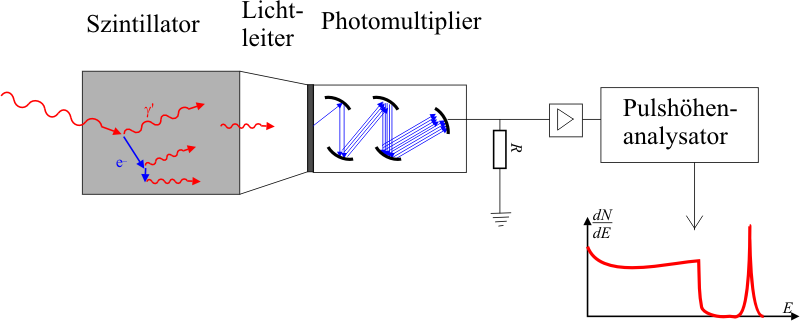
\includegraphics{Bilder/Szint.png}
 \caption{Aufbau Szintillationsdetektor }
  \end{figure}
 Quelle: https://de.wikipedia.org/wiki/Szintillationsz\%C3\%A4hler
 \begin{figure}[H]
 \center
 \includegraphics[scale=0.5]{Bilder/skizze1.jpg}
 \caption{Gesamter Versuchsaufbau}
 \end{figure} 
 \newpage
 \section{\underline{Messdaten}}
 
  Die Messdaten für Aufgabe 2 sind unter anderem auf dem USB-Stick von Tassilo Scheffler gespeichert (Ordner: TASSILO/messungen). 
   Dort ist auch das Änderungsdatum des 15.03.2018 ersichtlich. Weiterhin sind Messungen unter dem Link \\ \url{https://github.com/clerusch/gp1/tree/master/gammaspektroskopie}\\ ersichtlich. Die Dateien von dem USB-Stick wurden jedoch erst später hochgeladen.
   
 \begin{table}[h]
 \caption{\"Aquivalenzdosiswerte}
 \centering
 \begin{tabular}{c|c}
 Ort &  gemessene \"Aquivalenzdosis in $\mu$Sv/h \\ \hline
 Luft &  0.2\\
 0.5m Abstand zu $^{60}$Co-Präparat &  0.5\\
 
 \end{tabular}
\end{table}
 \begin{table}[h]
 \caption{Peaks der Diagramme 4, 5, 6 und 7}
 \centering
 \begin{tabular}{c|c|c|c|c}
 Element &  Kanalposition Peak 1 & Kanalposition Peak 2 & Standardabweichung $\sigma$ Peak 1 & $\sigma$ Peak 2 \\ \hline
 $^{60}$Co &  3290 & 3663 & 114 & 91.6\\
 $^{22}$Na & 1499 & 3542 & 63.5 & 101\\
 $^{137}$Cs & 1922 & - & 69.7 & -\\
 $^{241}$Am & 196 & - & 12.8 & -\\

 
 \end{tabular}
\end{table}

\begin{table}[h]
\caption{Absorption von $\gamma$ - Quanten mithilfe von Eisen bei $^{60}$Co}
\centering
\begin{tabular}{c|c|c}
 Breite des Eisens & Impulse des Photoeffekt-Peaks & Fehlerwert $\sqrt{Impulse}$\\\hline
 0 & 5078 & 71.26\\
 5 & 4723 & 68.72\\
 10 & 4049 & 63.63\\
 15 & 3538 & 59.48\\
 20 & 3129 & 55.94\\
 25 & 2851 & 53.39\\
 30 & 2523 & 50.23\\
 35 & 2208 & 46.99\\
 40 & 2035 & 45.11\\
 45 & 1815 & 42.60\\
\end{tabular}
\end{table}

\begin{table}[h]
\caption{Absorption von $\gamma$ - Quanten mithilfe von Blei bei $^{60}$Co}
\centering
\begin{tabular}{c|c|c}
 Breite des Bleis & Impulse des Photoeffekt-Peaks & Fehlerwert $\sqrt{Impulse}$\\\hline
 0 & 5028 & 70.91\\
 3 & 3824 & 61.84\\
 6 & 3147 & 56.10\\
 9 & 2544 & 50.44\\
 12 & 2042 & 45.19\\
 15 & 1725 & 41.53\\
 18 & 1434 & 37.87\\

\end{tabular}
\end{table}
\newpage
\begin{figure}[H]
\includegraphics[scale=0.5]{Bilder/Cs137.png}
\caption{\label{f:myfig} Caesium-137 Spektrum}
\end{figure}
\begin{figure}[H]
\includegraphics[scale=0.5]{Bilder/Na22.png}
\caption{\label{f:myfig} Natrium-22 Spektrum}
\end{figure}
\begin{figure}[H]
\includegraphics[scale=0.5]{Bilder/Co60.png}
\caption{\label{f:myfig} Cobalt-60 Spektrum}
\end{figure}
\begin{figure}[H]
\includegraphics[scale=0.5]{Bilder/Am241.png}
\caption{\label{f:myfig} Americium-241 Spektrum}
\end{figure}
\newpage
\newpage
\section{\underline{Auswertung}}
  \subsection{Aufgabe 1}
   gemessene \"Aquivalenzdosis der Luft: 0.2 $\mu$Sv/h \\
   gemessene \"Aquivalenzdosis durch $^{60}{Co}$ bei 0.5 m Entfernung zu dem Messgerät: 0.5 $\mu$Sv/h \\
   \"Aquivalenzdosis/Jahr = Dosis/h $\cdot$ 24 $\cdot$ 365 = Dosis/h $\cdot$ 8.760 \\
   $\Rightarrow$ \"Aquivalenzdosis der Luft/Jahr = 1.752 mSv, $^{60}{Co}$-\"Aquivalenzdosis/Jahr = 4.380 mSv \\
   
     \subsection{Aufgabe 2}
     Die Aufnahme der $\gamma$ - Spektren erfolgte in den Abbildungen 4, 5, 6 und 7.
   Das Diagramm 1 (Kalibrierung) wurde mithilfe der gemessenen Photopeaks in Tabelle 1 und der vorgegebenen Werte aus den Zerfallsschemen (Abb. 1) konstruiert. 
   Die Grenzgerade ergibt sich aus der Standardabweichung der Peaks.
    Von nun an k\"onnen Kanalnummern hiermit Energien zugeordnet werden.
   
  \subsection{Aufgabe 3}
   Der Vernichtungsstrahlungs-Peak von $^{22}{Na}$ liegt nach Tabelle 2 bei Kanalnummer 1499. Aus dem Kalibrierungsgraphen liest man für diesen Kanal eine Energie von E = (0.53 $\pm$ 0.02)MeV ab. Der Fehler bestimmt sich aus der Grenzgeraden aus (0.55 - 0.53)MeV.
   Der theoretische Vergleichswert wird mithilfe von Gleichung $\ref{Einstein}$ bestimmt. Dieser ergibt dann E = 0.511 MeV.
   \subsection{Aufgabe 4}
   Mit der Gleichung $\ref{Auflosung}$ und der Tabelle 2 ergibt sich f\"ur das Aufl\"osungsverm\"ogen von dem verwendeten Szintillationsdetektor bei $^{137}$Cs:
   \begin{equation}
   	A = \frac{69.7}{1922} = 0.036 = 3.6\%
   \end{equation}
  \subsection{Aufgabe 5}
   Die Compton-Kante liegt bei unserer Abbildung 5 bei Kanalnummer 1408, also nach Kalibrierungsdiagramm bei (0.50 $\pm$ 0.02) MeV.
   Der theoretische Vergleichswert nach der Streuformel (Gleichung $\ref{Streuformel}$) ergibt mit dem Zerfallsschema von dem Caesiumisotop, welches $E_0 = 0.662MeV$ liefert. Au\ss erdem wird der Wert $m_0c^2 = 0.511MeV$ Aufgabe 3 entnommen.
   \begin{equation}
    T = \frac{0.662 MeV}{1+\frac{0.511 MeV}{(1-cos \pi)\cdot 0.662 MeV}} = 0.478 MeV
   \end{equation}
  \subsection{Aufgabe 6}
  Hierfür wurden nur die Kanäle selektiert, welche dem Photopeak angehörig sind. Die Impulse in diesem Bereich wurden gemessen und in den Tabellen 3 und 4 niedergetragen. 
  Um den Absorptionskoeffizienten zu berechnen benötigt man Gleichung $\ref{Absorption}$, da diese Werte aus den angelegten Diagrammen ????? ersichtlich sind.
  Es wurde jeweils für einen beliebigen Punkt der Ausgleichsgraden die Anzahl der Impulse und die Dicke x notiert.
  Es ergibt sich somit:
  \begin{align}
  	\mu_{Eisen} = \frac{ln(5078)-ln(3250)}{20mm}= 0.022 \frac{1}{mm}
  	\\\mu_{Blei} = \frac{ln(5028)-ln(2600)}{9mm}= 0.073 \frac{1}{mm}
  \end{align}
  Die Halbwertsdicke ergibt sich aus Gleichung $\ref{HWD}$ mit dem bereits errechneten Wert $\mu$:
  \begin{align}
  	x_{0.5,Eisen} = \frac{ln(2)}{0.022 \frac{1}{mm}} = 31.51mm
  	\\x_{0.5, Blei} = \frac{ln(2)}{0.073 \frac{1}{mm}} = 9.50mm
  \end{align}
  
  \subsubsection{Fehlerbetrachtung}  
  Der betrachtete Fehler ergibt sich aus der Grenzgeraden und ist für die Anzahl der Impulse gültig. 
  Aus Tabelle 3 und 4 wird der Fehlerwert f\"ur $I_0$ abgelesen.
  Der Fehler für die Dicke x ist nicht bekannt.
  Wie die Fehler der Anzahl der Impulse den Absorptionskoeffizienten bzw. die Halbwertsdicke beeinflusst, bestimmt die Gau\ss sche Fehlerfortpflanzung.
  \begin{align}
  	\Delta \mu &= \sqrt{\left(\frac{1}{I_0x}\Delta I_0\right)^2+\left(\frac{-1}{Ix}\Delta I\right)^2}
  	\\\Rightarrow \Delta \mu_{Eisen} &= \sqrt{\left(\frac{1}{5078\cdot 20mm} \cdot 71.26\right)^2+\left(\frac{-1}{3250\cdot 20mm}\cdot 70\right)^2}= 0.0013 \frac{1}{mm}
  	\\\Rightarrow \Delta \mu_{Blei} &= \sqrt{\left(\frac{1}{5028\cdot 9mm} \cdot 70.91\right)^2+\left(\frac{-1}{2600\cdot 9mm}\cdot 70\right)^2}= 0.0034 \frac{1}{mm}
\end{align}   
Der Fehlerwert für die Halbwertsdicke ergibt sich dann aus dem Fehlerwert für den Absorptionskoeffizienten:
\begin{align}
	\Delta x_{0.5} &= \sqrt{\left(\frac{-ln(2)}{\mu^2}\Delta \mu\right)^2}
	\\\Rightarrow \Delta x_{0.5,Eisen} &= \frac{ln(2)}{0.022\frac{1}{mm}^2}\cdot 0.0013 \frac{1}{mm} = 1.9mm
	\\\Rightarrow \Delta x_{0.5,Blei} &= \frac{ln(2)}{0.073\frac{1}{mm}^2}\cdot 0.0034 \frac{1}{mm} = 0.44 mmm
\end{align}
\newpage
   \section{Diskussion}
   In \underline{Aufgabe 1} hat man mithilfe des \"Aquivalenzdosisleistungsmessger\"ates die ungef\"ahre K\"orperdosis pro Jahr von 1.75 mSv in der Luft und von 4.38 mSv in 0.5m Entfernung zu dem Cobalt-Präparat ermittelt. 
   Dieser Wert überschreitet die Richtlinien f\"ur die Strahlenbelastung, die ein normaler B\"urger abbekommen darf pro Jahr. Dies ist jedoch unproblematisch, 
   da der Aufenthalt in dem Versuchsraum nur sehr gering war, im Vergleich zu einem Jahr und weil man sich bei solchen noch gerinf\"ugigen Mengen an Strahlung noch 
   keine gro\ss en Sorgen um seine Gesundheit machen muss, soweit man vorsichtig damit umgeht. \\
   F\"ur \underline{Aufgabe 2} wurden die Abbildungen 3, 4 und 5 angelegt mithilfe von einer 5 min\"utigen Messung. 
   Man erkennt hierbei die Photoeffekt- und Vernichtungsstrahlungs-Peaks sehr gut und auch die Compton-Kante f\"ur das Caesiumisotop l\"asst sich gut erkennen. 
   Das angelegte Kalibrierungsdiagramm ergibt dementsprechend auch einen linearen Verlauf. Die Messungen sind also gut verlaufen.\\
   Der Vernichtungsstrahlungs-Peak von der $\gamma$-Strahlung von $^{22}$Na wurde in \underline{Aufgabe 3} ausgewertet. 
   Dieser ergab mit Vergleich des Kalibrierungsdiagrammes einen Wert von (0.53 $\pm$ 0.02)MeV. 
   Im Vergleich zu den theoretisch bestimmten 0.511 MeV ist dieser Wert also identisch mit dem theoretischen Wert, 
   da der theoretische Wert in dessen Fehlerintervall liegt. Die Messung ist somit sehr gut verlaufen. \\
   \underline{Aufgabe 4} befasste sich mit der Ermittlung des Aufl\"oseverm\"ogens des Szintillationsdetektors, welcher 3.6 \% ergab.
   Dieser Wert befindet sich ungef\"ahr in der normalen Gr\"o\ss enordnung f\"ur Szintillationsdetektoren von ca. 10\%. 
   Somit ist das Aufl\"osungsverm\"ogen des benutzten Detektors sogar ein St\"uck besser. \\
   In \underline{Aufgabe 5} wurde die Compton-Kante von dem Caesiumisotop ausgewertet. Messtechnisch wurden mithilfe des Zerfallsdiagrammes und des Kalibrierungsdiagrammes 
   ein Wert von (0.50 $\pm$ 0.02) MeV ermittelt. 
   Der theoretische Wert ergibt sich aus der Streuformel in Gleichung $\ref{Streuformel}$ und wird zu 0.478 MeV errechnet. 
   Daraus schlussfogert man, dass der gemessene Wert im Vergleich mit dem errechneten Wert vertr\"aglich ist. Eine Fehlerquelle daf\"ur k\"onnte die Breite der Compton-Kante sein, welche sich \"uber einige Kan\"ale erstreckt. Alles in allem isst diese Aufgabe mit Versuch aber auch gut gelungen.\\
   Die Halwertsdicke und die Absorptionskoeffizienten von Blei und Eisen wurden in \underline{Aufgabe 6} bestimmt mithilfe von Abschirmung des Photoeffekt-Peaks bei dem radioaktiven $^{137}$Cs. Es ergaben sich die Werte:
   \begin{align}
   	\mu_{Eisen} &= (0.022 \pm 0.002) \frac{1}{mm}\\
   	\mu_{Blei} &= (0.073 \pm 0.004) \frac{1}{mm}\\
   	x_{0.5,Eisen} &= (32 \pm 2)mm\\
   	x_{0.5,Blei} &= (9.5 \pm 0.5)mm\\   	
   \end{align}
   Theoretische Vergleichswerte findet man zum Beispiel auf \url{www.onmeda.de}, welches Werte von
   \begin{align}
   	x_{0.5,Eisen} &= 10.6 mm\\
   	x_{0.5,Blei} &= 4.22 mm
   \end{align}
   aussagt bei ca. 0.5 MeV Gammastrahlung. Dieser Wert liegt ein wenig unter der verwendeten Gammastrahlung. 
   Die theoretischen Werte sind jedoch trotzdem signifikant unterschiedlich zu den ermittelten Werten, was eventuell daran liegt, dass zwischen dem Pr\"aparat und dem Szintillationsdetektor auch etwas Luft war, 
   da mit einer 45mm dicken Eisenschicht angefangen wurde. Die Messung von 0mm Eisen zwischen Pr\"aparat und Detektor hatte somit eine 45mm dicke Luftschicht dazwischen. 
   Diese sollte jedoch die $\gamma$-Strahlung nicht so sehr beeinflussen wie es in diesem Versuch geschehen ist. 
   Dementsprechend m\"ussen noch andere unbekannte Einf\"usse eingewirkt haben.
   Der Versuch ist deshalb nur teils gelungen, da wenigstens die Halbwertsdicke von Blei deutlich unter der von Eisen liegt, 
   was einen durchaus sinnvollen Bezug darstellt.
\end{document}
